\section{Life-cycle analysis}
\paragraph{}
The previous approach was detecting topics in short time periods and revealing relations between them. Here, we consider the recurrent topics that would happen several times in the whole study period or would last numerous time periods. For this themes, the goal is to be able to determine how the importance of a theme is varying over time.

\subsection{Overall Method}
\subsubsection*{Input}
The life-cycle analysis considers longer time periods than the transition graph but fewer themes. It thus requires additional input :
\begin{itemize}
\item The full sequence of words as they chronologically appear in the articles,
\item The background model,
\item The themes we are studying.
\end{itemize}

\paragraph{}
To be able to perform the themes strength analysis, the themes first need to be extracted. These themes are \emph{trans-collection themes}. The most straightforward way to find them would be to perform themes detection over very long durations (several years or decades), but the performance of the EM algorithm does not allow that. Indeed, the EM algorithm is well parallelized and efficient when processing many short time periods but a single long window of time would be analyzed sequentially which would require a huge amount of time. Two work-around strategies have been found for this issue :
\begin{itemize}
\item Perform the analysis over several shorter time periods and retain only the themes that have the highest probability. Then try to analyze whether some last longer than other or whether some are recurrent in time.
\item Perform the two steps : EM algorithm and evolutionary transitions computation. This will leave us with a graph of temporal dependencies between themes. Then the trans-collection themes can be identified as the longest connected components in our graph. This allows us to detect the themes that last long or that are recurrent. Finally to obtain the trans-collection themes, the probabilities of the short themes are averaged.
\end{itemize}

\paragraph{}
We had time only to implement the first of these two options. Although the second one seems worth trying, the first one gave us satisfying results, so our focus was more on the algorithm related to the Hidden Markov Models.

\subsubsection*{Algorithm}
\paragraph{}
The main idea of this life-cycle analysis is to consider that the full text of the articles was generated by a Markov Model which states are the background model and the themes. We are then interested in what hidden states were actually visited during the generation of the observation sequence. The procedure consists of the following steps :
\begin{itemize}
\item Train the HMM, i.e. learn its parameters using the Baum-Welch algorithm.
\item Decode the observation sequence by finding the most probable sequence of hidden states that generated the observation sequence. This is done using the Viterbi algorithm.
\item Compute the scores of the studied themes over time by counting the number of occurrences of each theme in the decoded sequence.
\end{itemize}

\begin{figure}[H]
\begin{center}
\begin{tikzpicture}[>=stealth',shorten >=1pt,auto,node distance=4cm]
  \node[state] (bg)      {$Background$};
  \node[state]         (t1) [above left of=bg]  {$Theme 1$};
  \node[state]         (t2) [above right of=bg] {$Theme 2$};
  \node[state]         (t3) [below of=bg] {$Theme 3$};

  \path[->]          (bg)  edge [loop right] node {0.9} (bg);
  \path[->]          (bg)  edge [bend left] node {0.05} (t1);
  \path[->]          (bg)  edge [bend right] node {0.03} (t2);
  \path[->]          (bg)  edge [bend left] node {0.02} (t3);
  \path[->]          (t1)  edge [loop above] node {0.6} (t1);
  \path[->]          (t2)  edge [loop above] node {0.5} (t2);
  \path[->]          (t3)  edge [loop below] node {0.4} (t3);
  \path[->]          (t1)  edge [bend left] node {0.4} (bg);
  \path[->]          (t2)  edge [bend right] node {0.5} (bg);
  \path[->]          (t3)  edge [bend left] node {0.6} (bg);
 
 
\end{tikzpicture}
\label{fig:hmm}
 \caption{Example of a HMM with 4 states (analyzing 3 themes)}
\end{center}
\end{figure}

\subsection{Parallel Baum-Welch Algorithm}
\paragraph{}
The Baum-Welch algorithm is a classic algorithm to train a Hidden Markov Model given an observed sequence. The algorithm is capable of estimating the initial probability distribution, the transition probability distribution, and the emission probability distribution. In its most-basic (but efficient) forward-backward version as presented in \cite{rabiner1989tutorial} for example, the algorithm computes some probabilities from the beginning of the observed sequence to the end, and some other probabilities from the end of the observed sequence to the beginning. It has the advantage to be fast compared to other algorithms like the forward only or backward only presented in \cite{turin1998unidirectional} but uses a lot of memory, and is sequential by nature. Some work has to be done to make it parallel on the observed sequence (as presented for example in \cite{turin1998unidirectional}), or precise (as presented for example in \cite{rabiner1989tutorial}). However, the combination of accuracy and parallel acceleration over the observed sequence is a real challenge. Thus, we extended the known algorithms to design a precise and parallel algorithm for very long observation sequences.

\paragraph{}
Our algorithm enabled us to train our Hidden Markov Model over a sequence of more than 500 million observations on a cluster of thousands of processors using Spark. It uses more memory than the original forward-backward version and also makes more computations, but can be run on as many cores as available. We will present in the rest of this section the original forward-backward algorithm, the precise variant, and our precise parallel algorithm.

\paragraph{}
In all the rest of this section, we use the same notations and definitions as on the Wikipedia (English) article of the Baum-Welch algorithm. We first present the original algorithm as on the Wikipedia article, then present the precise version suggested in \cite{rabiner1989tutorial}, then briefly the parallel version suggested in \cite{turin1998unidirectional}, and ultimately our precise parallel version which is built upon the two ideas.

\subsubsection*{Hidden Markov Model}
(This section is a mere copy of definitions used in \cite{wiki:BaumWelch_algorithm}).
\paragraph{}
Let $X_t$ be the hidden variables (each taking $N$ possible values) and $Y_t$ the observation variables (each taking $M$ possible values). We assume that the Markov chain is homogeneous, that is $P(X_t|X_{t-1})$ is independent from the time $t$.
It is therefore possible to define the transition probability matrix $A = \{a_{i,j}\} = P(X_t = j | X_{t-1} = i)$.
We can define the initial probability distribution as $\pi_i = P(X_1=i)$ and the emission probabilities as $b_j(y_t) = P(Y_t = y_t | X_t = j)$. Usually is defined the emission probability matrix $B = \{b_j(y_i)\} = P(Y_i=y_i | X_j)$.

\paragraph{}
With such definitions, we can define the parameters of a Hidden Markov Model as the triplet $\Theta = (A, B, \pi)$, where $A$ is the transition probability matrix, $B$ is the emission probability matrix, and $\pi$ is the initial probability distribution.

\subsubsection*{Baum-Welch Algorithm}
(This section is a mere copy of the notations and definitions used in \cite{wiki:BaumWelch_algorithm}).
\paragraph{}
The Baum-Welch algorithm is an algorithm using the Expectation-Maximization principle to find the parameters $\Theta^*$ such that $P(Y_1,...,Y_T| \Theta^* )$ is a local maximum.
In its forward-backward version, it is necessary to compute first during the forward procedure the coefficients $\alpha_i(t) = P(Y_1=y_1,...,Y_t = y_t, X_t = i | \Theta )$ and then it is necessary to compute the coefficients $\beta_i(t) = P(Y_{t+1}=y_{t+1},...,Y_T = y_T| X_t = i, \Theta )$.
\paragraph{}
Once those forward and backward coefficients are computed, it is possible to update the initial distribution, transition probability matrix and the emission matrices, as shown in \cite{rabiner1989tutorial} or \cite{wiki:BaumWelch_algorithm}. We have used this forward-backward algorithm as the starting point of our algorithm.

\subsubsection*{Precise Forward-Backward algorithm}
\paragraph{}
The original Baum-Welch algorithm depicted in the previous section suffers from precision problems (underflows) when the size of the sequence size grows up. As presented in \cite{rabiner1989tutorial}, one way to fix that is by defining a family of scaled coefficients $\hat{\alpha}_i(t)$ and $\hat{\beta}_i(t)$ defined by the relations:
\begin{equation}
\begin{cases}
\bar{\alpha}_i(1) = \pi_i b_i(y_1) & \\
\bar{\alpha}_i(t) = b_i(y_t)\sum_{j=1}^{N}{a_{j,i}\bar{\alpha}_j(t-1)} & \text{for t \textgreater 1} \\
c_t = \frac{1}{\sum^N_{j=1} \bar{\alpha}_j(t)} & \\
\hat{\alpha}_i(t) = c_t \bar{\alpha}_i(t) & \text{for all t}
\end{cases}
\end{equation}
And
\begin{equation}
\begin{cases}
\bar{\beta}_i(T) = 1 & \\
\bar{\beta}_i(t) = b_j(y_{t+1})\sum_{j=1}^{N}{a_{i,j}\hat{\beta}_j(t+1)} & \text{for t \textless T} \\
\hat{\beta}_i(t) = c_t \bar{\beta}_i(t)
\end{cases}
\end{equation}
The update rules are described in \cite{rabiner1989tutorial}.

\subsubsection*{Precise parallel Forward-Backward algorithm}
\paragraph{}
As described in \cite{turin1998unidirectional}, it is possible to design a parallel forward-backward algorithm from the traditional forward-backward algorithm as the relations defining the forward and backward coefficients are linear. To do so, it is necessary to use matrix computations. However, the way scaling is done in the precise version of algorithm seems to prevent the use of this idea to make a precise and parallel algorithm. This is not the case, and we show how in this section.

\paragraph{}
In the previous section, the relations defining the scaled forward coefficients can be in fact reinterpreted as the following relations:
\begin{equation}
\begin{cases}
\bar{\alpha}_i(1) = \pi_i b_i(y_1) & \\
\bar{\alpha}_i(t) = b_i(y_t)\sum_{j=1}^{N}{a_{j,i}\bar{\alpha}_j(t-1)} & \text{for t \textgreater 1} \\
\hat{\alpha}_i(t) = c_t \bar{\alpha}_i(t) & \text{for all t} \\
\text{with } c_t \text{ such that } \sum_{j=1}^{N}{\hat{\alpha}_j(t)} = 1 & \text{for }t \ge 1
\end{cases}
\end{equation}

\paragraph{}
While it was previously not possible to design a parallel algorithm due to the definition of the $c_t$ coefficients (hindering the parallel computation of the $\hat{\alpha}_i(t)$ coefficients), it is now possible. If we define the matrices $\bar{Fo}(t_1 \rightarrow t_1 + 1)$ (one step forward matrices), the matrices $\bar{Ba}( t_1 \leftarrow t_1 + 1)$ (one step backward matrices), the vectors $\bar{\alpha}(t)=(\bar{\alpha}_i(t))$, and the vectors $\bar{\beta}(t)=(\bar{\beta}_i(t))$ with the following relations:
\begin{equation}
\begin{cases}
\bar{Fo}( t - 1 \rightarrow t) =  \{b_i(y_{t+1})a_{ji}\} & \\
\bar{\alpha}(1) =  (\pi_i b_i(y_1))_{1 \le i \le N} & \\
\bar{\alpha}(t) =  \bar{Fo}( t - 1 \rightarrow t) \hat{\alpha}_i(t - 1) & \text{for t \textgreater 1} \\
\hat{\alpha}(t) = c_t \bar{\alpha}(t) &
\end{cases}
\begin{cases}
\bar{Ba}( t \leftarrow t + 1) = \{b_j(y_{t+1})a_{ij}\} & \\
\bar{\beta}(T) = (1)_{1 \le i \le N} & \\
\bar{\beta}(t) =  \bar{Ba}( t \leftarrow t + 1) \hat{\beta}(t + 1) & \text{for t \textless T} \\
\hat{\beta}(t) = c_t \bar{\beta}(t) &
\end{cases}
\end{equation}

\paragraph{}
It is possible to parallelize with some more general matrices $\bar{Fo}(t_1 \rightarrow t_2)$ (forward matrices), $\bar{Ba}(t_1 \leftarrow t_2)$ (backward matrices), $\hat{Fo}(t_1 \rightarrow t_2)$ (precise forward matrices), $\hat{Ba}(t_1 \leftarrow t_2)$ (precise backward matrices), following these constitutive relations:

\begin{equation}
\begin{cases}
\bar{Fo}( t - 1 \rightarrow t) =  \{b_i(y_{t+1})a_{ji}\} & \\
\bar{Fo}( t_1 \rightarrow t_3) =   \bar{Fo}( t_2 \rightarrow t_3) \hat{Fo}( t_1 \rightarrow t_2)& \\
\hat{Fo}( t_1 \rightarrow t_3) =   \hat{Fo}( t_2 \rightarrow t_3) \hat{Fo}( t_1 \rightarrow t_2)& \\
\bar{\alpha}(t_2) =  \bar{Fo}( t_1 \rightarrow t_2) \hat{\alpha}(t_1) & \\
\hat{\alpha}(t_2) =  \hat{Fo}( t_1 \rightarrow t_2) \hat{\alpha}(t_1) &
\end{cases}
\begin{cases}
\bar{Ba}( t \leftarrow t + 1) = \{b_j(y_{t+1})a_{ij}\} & \\
\bar{Ba}(t_1 \leftarrow t_3) = \bar{Ba}(t_1 \leftarrow t_2) \hat{Ba}(t_2 \leftarrow t_3) & \\
\hat{Ba}(t_1 \leftarrow t_3) = \hat{Ba}(t_1 \leftarrow t_2) \hat{Ba}(t_2 \leftarrow t_3) & \\
\bar{\beta}(t_1) =  \bar{Ba}( t_1 \leftarrow t_2) \hat{\beta}(t_2) & \\
\hat{\beta}(t_1) =  \hat{Ba}( t_1 \leftarrow t_2) \hat{\beta}(t_2) & \\
\end{cases}
\end{equation}

\paragraph{}
It is possible to compute in parallel as we can choose any families of matrices $\hat{Fo}(t_1 \rightarrow t_2)$ and $\hat{Ba}(t_1 \leftarrow t_2)$ just guaranteeing that
\begin{equation}
\begin{cases}
\hat{Fo}( t - 1 \rightarrow t) = \frac{\bar{Fo}( t - 1 \rightarrow t)}{\norm{\bar{Fo}( t - 1 \rightarrow t)}_1} & \\
\hat{Fo}( t_1 \rightarrow t_3) =   \frac{\hat{Fo}( t_2 \rightarrow t_3) \hat{Fo}( t_1 \rightarrow t_2)}{\norm{\hat{Fo}( t_2 \rightarrow t_3) \hat{Fo}( t_1 \rightarrow t_2)}_1}& \\
\end{cases}
\begin{cases}
\hat{Ba}(t \leftarrow t+1) = \frac{\bar{Ba}(t \leftarrow t+1)}{\norm{\bar{Ba}(t \leftarrow t+1)}_1} & \\
\hat{Ba}(t_1 \leftarrow t_3) = \frac{\hat{Ba}(t_1 \leftarrow t_2) \hat{Ba}(t_2 \leftarrow t_3)}{\norm{\hat{Ba}(t_1 \leftarrow t_2) \hat{Ba}(t_2 \leftarrow t_3)}_1} & \\
\end{cases}
\end{equation}

\paragraph{}
Which we can generate with any implementation of a parallel scan (primitive introduced by \cite{blelloch1990prefix}, with an implementation for GPUs in \cite{sengupta2008efficient} for example) starting from the set of matrices $\hat{Fo}( t - 1 \rightarrow t)$. Computing \emph{a posteriori} the $c_t$ coefficients, and then doing another parallel scan starting from the set $\hat{Ba}(t \leftarrow t+1)$. The rest of the algorithm can be easily done in a parallel fashion.

\subsubsection*{Precise parallel Forward-Backward algorithm complexity}
\paragraph{}
The total work required now to do an update step with this algorithm is $O(T(N^3 + NM))$ ($O(TN^3)$ to compute the matrices, $O(N)$ to update the initial probability distribution, $O(TN^2)$ to update the transition matrix, $O(TNM)$ to update the emission matrix). But the running time can be lowered to $O(ln(T)(N^3 + NM))$ by applying the parallel scan and performing matrix computations sequentially (it can be lowered again by making matrix multiplications in parallel). The memory complexity of the algorithm increases to $O(TN^2 + NM)$ compared to the $O(TN + NM)$ of the sequential forward backward algorithm.

\subsubsection*{Precise parallel Forward-Backward algorithm performance}
\paragraph{}
This algorithm enabled us to process sequences of the order of 500 million observations on a cluster of a thousand nodes with $N=10$ and $M=5000$, which was not possible on a single machine due to memory and time limitations. We also tried an implementation on GPUs of this algorithm and were able to have a 10x boost on an AMD HD7870 GPU compared to an Intel Core I7 4510U CPU when doing double precision computations.

\paragraph{Adaptations to our problem}
As in our problem, we modeled the HMM with very few transitions between states (we only have transitions to or from the background model to a theme), the transition matrix is very sparse. We also used this fact to lower the complexity of the algorithm by a factor of $N$, letting us to keep more themes while doing the training of HMM phase.

\subsection{Viterbi Algorithm and Scoring functions}
\paragraph{}
Training is from far the hardest task. Finding the most probable states sequences that generated a given observation sequence is quite straightforward using the Viterbi algorithm. A precise description of this algorithm can be found in \cite{rabiner1989tutorial}. We followed the algorithm quite closely, nevertheless two things are worth noting. To avoid troubles with double precision when probabilities come too close to zero, all the computations are done in log-space. And, although sequential by nature, our implementation uses Spark to split the sequence into blocks in order to prevent from using too much memory at once on the master node.

\paragraph{}
Computing the scores only consists in counting for each day the number of occurrences of each themes. We made the choice to keep the results in this form and to perform smoothing only when displaying them.

\subsection{Results}
\paragraph{}
Once these scores are computed, they can be displayed on the interface we implemented. Two compelling examples can be found in figures \ref{fig:resStrength1} and \ref{fig:resStrength2}.

\begin{figure}[H]
\centering
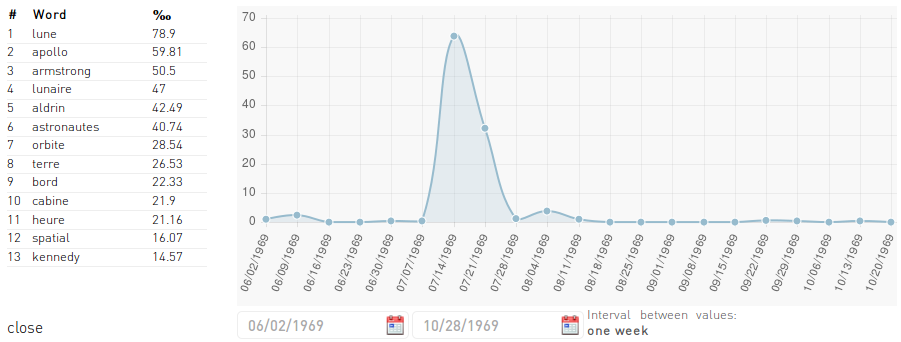
\includegraphics[width=0.9\textwidth]{images/apollo}
\caption{Strength of the theme concerning the Apollo mission over a period of five months}
\label{fig:resStrength1}
\end{figure}

\begin{figure}[H]
\centering
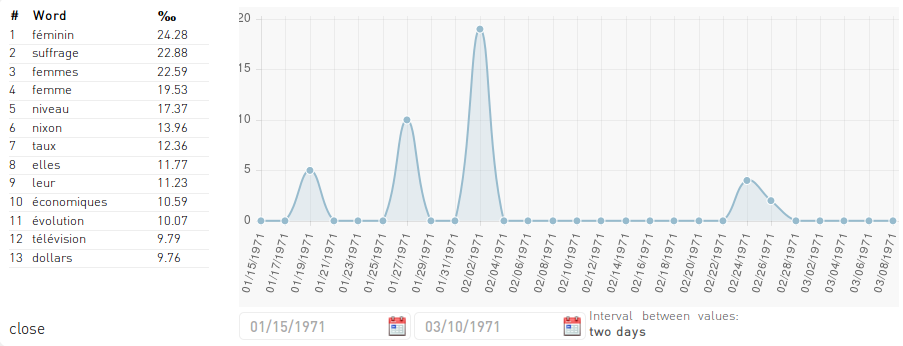
\includegraphics[width=0.9\textwidth]{images/voteFemmes}
\caption{Strength of the theme concerning women vote over a period of two months}
\label{fig:resStrength2}
\end{figure}
